\emph{Skirmishers} uses dotted mapsheets.
Dots are laid out in a hexagonal pattern, 1 inch apart, and 1 inch on the map represents 2.5 meters.
Units occupy a single dot on the mapsheet and may move between adjacent dots.

\begin{figure}[!h]
  \centering
  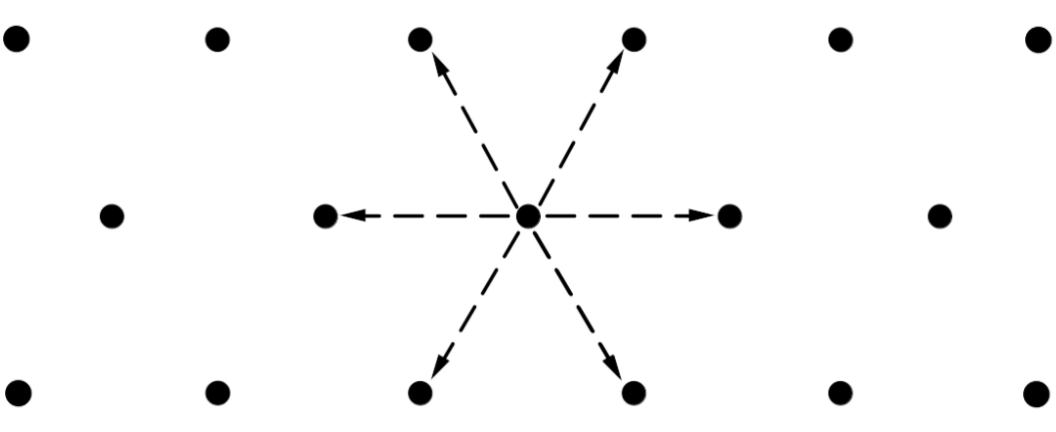
\includegraphics[alt='Sample dotted mapsheet', width=6.5in, height=3.66in]{img/Map.png}
  \caption*{Sample Map Section}
\end{figure}
